\section{Door Class Reference}
\label{classDoor}\index{Door@{Door}}
{\tt \#include $<$door.hpp$>$}

Inheritance diagram for Door::\begin{figure}[H]
\begin{center}
\leavevmode
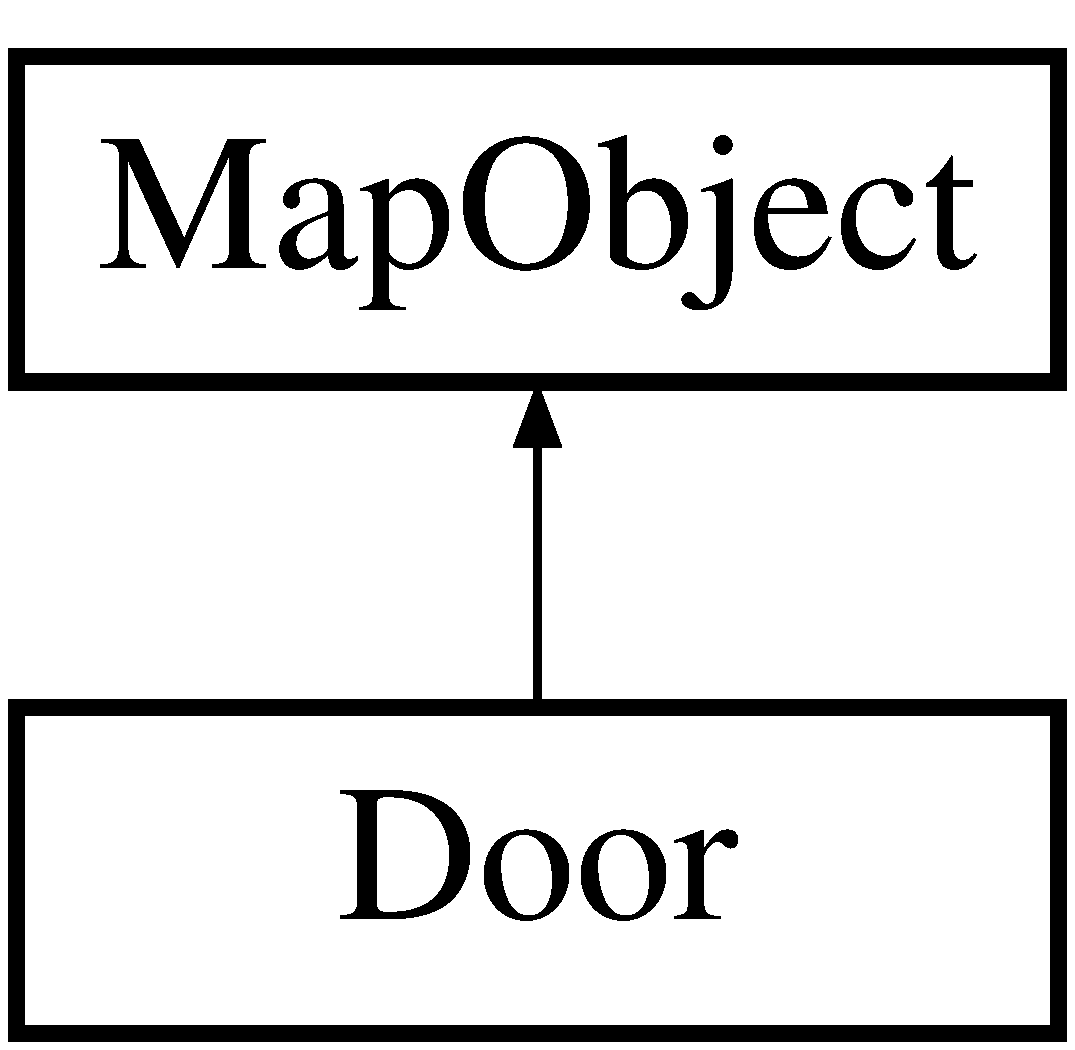
\includegraphics[height=2cm]{classDoor}
\end{center}
\end{figure}
\subsection*{Public Member Functions}
\begin{CompactItemize}
\item 
{\bf Door} (bool {\bf closed}, int {\bf closed\-Tile}, int {\bf open\-Tile})
\begin{CompactList}\small\item\em lock code \item\end{CompactList}\item 
virtual {\bf $\sim$Door} ()
\item 
virtual QString {\bf get\-Class\-Name} () const 
\item 
virtual bool {\bf is\-Obstacle} () const 
\item 
virtual bool {\bf is\-Bulletproof} () const 
\item 
virtual bool {\bf is\-Visionproof} () const 
\item 
bool {\bf is\-Closed} () const 
\item 
bool {\bf open} ()
\item 
bool {\bf close} ()
\item 
bool {\bf is\-Locked} () const 
\item 
void {\bf lock} ()
\item 
void {\bf unlock} ()
\end{CompactItemize}
\subsection*{Protected Attributes}
\begin{CompactItemize}
\item 
bool {\bf closed}
\item 
int {\bf closed\-Tile}
\item 
int {\bf open\-Tile}
\item 
bool {\bf locked}
\item 
QString {\bf code}
\end{CompactItemize}


\subsection{Constructor \& Destructor Documentation}
\index{Door@{Door}!Door@{Door}}
\index{Door@{Door}!Door@{Door}}
\subsubsection{\setlength{\rightskip}{0pt plus 5cm}{\bf Door} (bool {\em closed}, int {\em closed\-Tile}, int {\em open\-Tile})}\label{classDoor_a0}


lock code 

\index{Door@{Door}!~Door@{$\sim$Door}}
\index{~Door@{$\sim$Door}!Door@{Door}}
\subsubsection{\setlength{\rightskip}{0pt plus 5cm}$\sim${\bf Door} ()\hspace{0.3cm}{\tt  [virtual]}}\label{classDoor_a1}




\subsection{Member Function Documentation}
\index{Door@{Door}!close@{close}}
\index{close@{close}!Door@{Door}}
\subsubsection{\setlength{\rightskip}{0pt plus 5cm}bool close ()}\label{classDoor_a8}


\index{Door@{Door}!getClassName@{getClassName}}
\index{getClassName@{getClassName}!Door@{Door}}
\subsubsection{\setlength{\rightskip}{0pt plus 5cm}QString get\-Class\-Name () const\hspace{0.3cm}{\tt  [virtual]}}\label{classDoor_a2}




Implements {\bf Map\-Object} {\rm (p.\,\pageref{classMapObject_a0})}.\index{Door@{Door}!isBulletproof@{isBulletproof}}
\index{isBulletproof@{isBulletproof}!Door@{Door}}
\subsubsection{\setlength{\rightskip}{0pt plus 5cm}bool is\-Bulletproof () const\hspace{0.3cm}{\tt  [virtual]}}\label{classDoor_a4}




Reimplemented from {\bf Map\-Object} {\rm (p.\,\pageref{classMapObject_a3})}.\index{Door@{Door}!isClosed@{isClosed}}
\index{isClosed@{isClosed}!Door@{Door}}
\subsubsection{\setlength{\rightskip}{0pt plus 5cm}bool is\-Closed () const}\label{classDoor_a6}


\index{Door@{Door}!isLocked@{isLocked}}
\index{isLocked@{isLocked}!Door@{Door}}
\subsubsection{\setlength{\rightskip}{0pt plus 5cm}bool is\-Locked () const}\label{classDoor_a9}


\index{Door@{Door}!isObstacle@{isObstacle}}
\index{isObstacle@{isObstacle}!Door@{Door}}
\subsubsection{\setlength{\rightskip}{0pt plus 5cm}bool is\-Obstacle () const\hspace{0.3cm}{\tt  [virtual]}}\label{classDoor_a3}




Reimplemented from {\bf Map\-Object} {\rm (p.\,\pageref{classMapObject_a2})}.\index{Door@{Door}!isVisionproof@{isVisionproof}}
\index{isVisionproof@{isVisionproof}!Door@{Door}}
\subsubsection{\setlength{\rightskip}{0pt plus 5cm}bool is\-Visionproof () const\hspace{0.3cm}{\tt  [virtual]}}\label{classDoor_a5}




Reimplemented from {\bf Map\-Object} {\rm (p.\,\pageref{classMapObject_a4})}.\index{Door@{Door}!lock@{lock}}
\index{lock@{lock}!Door@{Door}}
\subsubsection{\setlength{\rightskip}{0pt plus 5cm}void lock ()}\label{classDoor_a10}


\index{Door@{Door}!open@{open}}
\index{open@{open}!Door@{Door}}
\subsubsection{\setlength{\rightskip}{0pt plus 5cm}bool open ()}\label{classDoor_a7}


\index{Door@{Door}!unlock@{unlock}}
\index{unlock@{unlock}!Door@{Door}}
\subsubsection{\setlength{\rightskip}{0pt plus 5cm}void unlock ()}\label{classDoor_a11}




\subsection{Member Data Documentation}
\index{Door@{Door}!closed@{closed}}
\index{closed@{closed}!Door@{Door}}
\subsubsection{\setlength{\rightskip}{0pt plus 5cm}bool {\bf closed}\hspace{0.3cm}{\tt  [protected]}}\label{classDoor_p0}


\index{Door@{Door}!closedTile@{closedTile}}
\index{closedTile@{closedTile}!Door@{Door}}
\subsubsection{\setlength{\rightskip}{0pt plus 5cm}int {\bf closed\-Tile}\hspace{0.3cm}{\tt  [protected]}}\label{classDoor_p1}


\index{Door@{Door}!code@{code}}
\index{code@{code}!Door@{Door}}
\subsubsection{\setlength{\rightskip}{0pt plus 5cm}QString {\bf code}\hspace{0.3cm}{\tt  [protected]}}\label{classDoor_p4}


\index{Door@{Door}!locked@{locked}}
\index{locked@{locked}!Door@{Door}}
\subsubsection{\setlength{\rightskip}{0pt plus 5cm}bool {\bf locked}\hspace{0.3cm}{\tt  [protected]}}\label{classDoor_p3}


\index{Door@{Door}!openTile@{openTile}}
\index{openTile@{openTile}!Door@{Door}}
\subsubsection{\setlength{\rightskip}{0pt plus 5cm}int {\bf open\-Tile}\hspace{0.3cm}{\tt  [protected]}}\label{classDoor_p2}




The documentation for this class was generated from the following files:\begin{CompactItemize}
\item 
{\bf door.hpp}\item 
{\bf door.cpp}\end{CompactItemize}
